\chapter{Discussion}

% \epigraph{\textit{This is the end. My only friend, the end.}}{--- \textup{Jim Morrison}}

\minitoc[n] % minitoc without title

The contributions of this thesis have been divided in two parts that, while they revolve around evolutionary robotics, are centered on very different problems. As such, we choose here to discuss and conclude on each part separately.

\section{Modeling the Evolution of Cooperation}

	\subsection{Summary of Contributions}

		In the first part of this thesis we have been interested in the influence of coordination on the evolution of mutualistic cooperation. We focused in particular on the proximate explanations of coordination and their impact on the ultimate evolution of cooperation. Most studies centered on cooperation have often been dedicated to explaining the stability of altruistic behaviours. Mutualistic actions in comparison have usually been ignored. However, while mutually beneficial actions do not raise any issue of stability, the origin of this type of cooperative behaviours is not trivial. Because they require coordination, the spread of a cooperative behaviour from an initial population of solitary individuals remains an open question. We thus were interested in the boostrap of mutually beneficial cooperation.

		To that end, we used evolutionary robotics as our modeling framework. Because we were interested in the origin of cooperative actions rather than their stability, the modeling of mechanistic constraints is critical. Namely, the convergence to a cooperative solution is impacted by the availability of mutations, i.e. the possibility for a particular mutant to appear in the population. While classical models in evolutionary biology are of great help in understanding the dynamics of the evolution of cooperation, they make critical assumptions with regards to the convergence towards a cooperative solution. This is what has motivated our choice to use individual-based modeling and evolutionary robotics in particular as a modeling method. In particular, evolutionary robotics allows to model the mapping between genotype and phenotype and thus study the proximate mechanisms at play in the evolution of cooperation.

		In a first study, we focused on the impact of modeling the mechanics of behaviour in the evolution of mutualistic cooperation. To that end we took inspiration from the game theoretical model of the stag hunt and studied the transition from a solitary equilibrium (hare hunting) to a cooperative equilibrium (stag hunting). We first revealed that there is a drastic difference between the results predicted by classical models in game theory and what we observed in evolutionary robotics. With a classical model, the transition to stag hunting always occured. In comparison, with a model in evolutionary robotics, this transition was nearly impossible. Furthermore, we showed that even under maximal genetic relatedness (i.e. individuals were clones of each other), the evolution of cooperation was still unlikely. We thus revealed that the mechanistic constraints are critical for the origin of cooperation in the stag hunt game. The evolution of cooperation is faced with a chicken and egg dilemma: for cooperation to be selected, it needs to be beneficial. Yet the success of the cooperative action requires that others evolved the capacity to coordinate, which is not beneficial on its own. If ones assumes that a single mutation can lead to the evolution of cooperation then we consider that the same mutation is responsible for both the modification of the preferred prey and the capacity to coordinate. We showed here that doing so hides part of the issue. Moreover we showed in our simulations that the individuals needed to evolve a complex behaviour in order to be able to coordinate. Therefore, it is necessary to take into account the mechanics of behaviours in order to fully understand the evolution of cooperation. This means that there is a need for complementary frameworks which model these mechanisms.

		In the second Chapter, we studied how the nature of coordination behaviours may impact the transition between collective equilibria. More precisely, we focused on the issue of selecting between multiple stable equilibria. When a collective equilibrium has emerged, no single mutant has a selective advantage to deviate from this equilibrium. As such, this raises the issue of the transition to the optimal equilibrium. Our goal was to study if individual selection alone could lead to the optimization of group-traits. To that end, we used a model of collective hunting where individuals could choose between two types of prey: boar (suboptimal prey) and stag (optimal prey). We revealed that the transition towards the optimal prey was impossible under simple environmental features (only one prey of each type). However, we revealed that results were different when more realistic assumptions about collective hunting are made. Surprisingly, when the environment was more complex (nine prey of each type), the switch to stag hunting could sometimes occur. Under such environmental conditions, it was necessary to collectively decide on which prey to hunt. This meant that the evolution of coordination was required to achieve cooperation. In consequence, each individual evolved the capacity to react to the other individual's behaviour. This meant that a mutant could indirectly change the behaviour of the group and thus lead to stag hunting. However, we observed that the coordination strategy evolved was a very symmetrical one where both individuals could adopt the same behaviour. We then increased the neural complexity of individuals. We showed that the transition to stag hunting was then highly facilitated. Furthermore, we revealed that individuals evolved a strongly asymmetrical coordination strategy through specialization: a leader/follower strategy. In this strategy, the follower only reacted to the behaviour of the leader which it tried to follow. This means that a mutation on the leader was sufficient to change the group's behaviour and thus reap the benefits of cooperative stag hunting. Additionally, we observed that this strategy was more efficient than the previous one in terms of rewards obtained. We thus revealed that the evolution of an individually adaptive strategy led to the transition to the optimal collective behaviour. Therefore, we showed that it was possible for individual selection alone to explain the optimization of group traits.

		In both of these studies, we thus revealed the critical role of coordination in the evolution of cooperation. In consequence, we demonstrated that it is indeed necessary to take the mechanics of coordination behaviours into account in order not to neglect crucial aspects of the evolutionary dynamics. Additionally, we also presented a general mechanism for the evolution of cooperation in the stag hunt. The boar we introduced in our study on the selection of equilibria could act as an evolutionary pathway in the stag hunt. Namely, this prey can be hunted alone but rewards more when it is hunted cooperatively, which is a realistic expectation for hunting in the natural world. As such, coordination and cooperation can initially be bootstrapped on this prey (because it is not as risky as hunting stags). Then, we showed that when coordination was present it was possible for individual selection to optimize the collective behaviour. In consequence, this could lead to the transition to the purely cooperative equilibrium: stag hunting.


	\subsection{Limits and Perspectives}

		\subsubsection{The evolution of communication}

			During this thesis, we have studied coordination strategies that did not require any direct communication between individuals. We wanted to study if coordination was possible without endowing individuals with communication capabilities. Indeed, we aimed at keeping the complexity of our robot model as low as possible so that we could focus on the basic mechanisms that could lead to the evolution of cooperation. More complex agents could beg the question of the role of the robots' capabilities on the observed phenomena. In particular, the goal behind the first part of our study was to compare classical models in evolutionary biology with modeling under an evolutionary robotics framework. As such, it was important that no particular design choice could alter the relevance of this comparison.

			We found that our robots were capable of coordination without any means of communication. Indeed, they could evolve a surprising behaviour which, while it was not the most efficient way to coordinate, allowed them to cooperate. In a way, we can make here a similar observation as Mitri and colleagues~\parencite{Mitri2009}. Namely, individuals could rely on indirect communication cues resulting from their embodiement. However we could also implement a more direct way for them to communicate. Communication is used in numerous different social species, among which we already gave the example of the spotted hyenas~\parencite{Drea2009a, Smith2010, Smith2012a}. They are capable of using signaling techniques and communication in order to achieve high level of coordination during collective hunting. As such, while the empasis of our second study was mainly put on division of labour, communication could deeply impact the nature of coordination behaviours. In consequence, we hypothesize that the evolution of communication strategies could affect the evolution of collective actions. Additionally, an interesting perspective would be to let the individuals evolve how to communicate from basic communication capabilities (e.g. the broadcast of a simple signal). As such, this could lead to coevolutionary dynamics between communication strategies and coordination behaviours.

			Moreoever, the evolution of communication has already been studied in several works in evolutionary robotics. We already mentioned in Chapter~\ref{chapter:model} that some have been interested in the general evolution of communication between foraging robots~\parencite{Floreano2007}, information suppression~\parencite{Mitri2009} or the role of historical contingencies on the evolution of signaling strategies~\parencite{Wischmann2012}. As with the evolution of cooperation, few have been interested in the role of communication among unrelated individuals. A notable counterexample is the work of Solomon et al.~\parencite{Solomon2012} who modeled communication strategies between hyenas. However, the impact of communication on the origin of mutualistic actions has not been studied.


		\subsubsection{Cooperation between bigger groups of agents}

			Our initial inspiration was the game theoretical framework of the stag hunt. As such interactions take place between only a pair of individuals. However, it could be interesting to increase the number of agents and to study how the evolutionary dynamics would change. In particular, in our second study we have been interested in the optimization of group-traits by way of individual selection. We showed that the transition between multiple equilibria could occur without any group-level mechanism. As we provided no evidence that our demonstration could be scaled up to more than two individuals, it could be argued that what we consider a group-trait is limited in this context. 

			However, we believe that similar results would be observed in larger groups of individuals. We even hypothesize that the results could be more explicit in this case. Let's imagine that we consider a scaled-up version of our study where interactions take place between $5$ agents. The stag would now require that the $5$ individuals cooperate together to reap the benefits of the hunt. Because the coordination of $5$ individuals is more challenging than that of a pair, the evolution of efficient coordination strategies would be even more favored. As such, the evolution of asymmetrical behaviours like the leader/follower should have a bigger impact on the transition towards the optimum. Indeed, it would be impossible for a single mutant to lead the group to stag hunting without an asymmetrical strategy. As of today, we have begun working on preliminary experiments where we increase the number of agents in our simulation (with groups of $3$, $4$ or $5$ robots). 

			% However, as of today we are faced with the fact that, given our parameters, it is challenging for the robots to evolve an efficient coordination strategy.


		\subsubsection{Online evolution}

			An interesting continuation of our work would be to model the evolution of mutualistic cooperation in a more ecologically realistic setup. More precisely, in the classical framework of evolutionary robotics we use an offline evolutionary algorithm. This initially means that there is a separation between the design of a robot and its deployment; robots are evolved in a different environment than the one where they are used. In comparison, under an online paradigm evolution occurs directly in the operational environment. The field of embodied evolution~\parencite{Watson2002} was created in order to address this question and in particular the issue of transferability that stems from evolving robots in an offline manner. As such, embodied evolution is mainly concerned with design questions. In our case, it would be interesting to use online evolution as another manner in which to model evolutionary phenomena. 

			Further, in the particular case of \emph{environment-driven} embodied evolution the selection pressure is driven by the environment. In classical ER (and embodied evolution), a fitness function is used to evaluate the performance of individuals and determine if they will produce offsprings. In this case, there is an obtective-driven selection pressure. This is different from the biological definition of fitness, where fitness is an \emph{a posteriori} evaluation of the reproductive sucess of a given individual. As such, a more realistic approach to the modeling of evolution would be to require that the individuals meet with each other in order to exchange genetic material~\parencite{Bredeche2010}. This is the principle of environment-driven embodied evolution. In consequence, a perspective would be to study the evolution of mutualistic cooperation under such paradigm. In this case an interesting feature is that the selection process also evolves.

			Few have focused on this aspect of biological modeling. Montanier and Bredeche investigated the evolution of altruism among a population of simulated robots under an online environment-driven algorithm~\parencite{Montanier2011, Montanier2013}. This way they could study the impact of genetical relatedness and dispersion on the emergence and stability of altruistic behaviours.


\section{Automatic Design of Collective Robots}

	\subsection{Summary of Contributions}

		In the second part of this thesis our goal was to study how to design the evolution of cooperation in evolutionary robotics. More precisely, we were interested in the impact of genetic team composition on the evolution of efficient coordination strategies in multirobot systems. Multirobot systems have multiple advantages in comparison to using a single robot among which robustness, efficiency and the capacity to achieve tasks that a single robot could not. However, because they require the control of several agents, they are also more challenging to design. In this context, multiple different architectures exist for multirobot systems and several ways to design the control of collective robots have been proposed. But while a popular and often efficient method has been to manually design the robots, there has been a strong interest in creating methods to automatically design them. Automatic design can lead to robots that better react to environmental changes and unknown environment. Additionally, some problems are simply nearly impossible to design in a manual fashion. In this context, we focused on evolutionary robotics as an approach to the automatic design of distributed robots.

		An open issue when designing cooperative robots in evolutionary robotics is team composition. Namely, the robots that constitute a team can be homogeneous or heterogeneous, whether in terms of morphology or control. Here we focused on the influence of team composition on the control of agents only. The classical approach in evolutionary robotics has been to use an homogeneous group of robots, where every individual comes from the same genotype. However, it is argued that heterogeneity could lead to more diverse behaviours between robots and thus generate higher efficiency.

		In the first Chapter of this part, we compared homogeneous and heterogeneous approaches on two criteria: evolvability and efficiency. We designed a collective foraging task inspired by the stag hunt where the individuals could forage two types of ressources: one that could be foraged alone and an other more rewarding that needed to be collected cooperatively. In this context, we use a restricted definition of evolvability where it corresponds to the capacity of a particular method to evolve cooperators. In comparison, efficiency refers to the performance of the cooperative solution w.r.t. ressources collected. We compared a clonal approach (i.e. where individuals are homogeneous) to two aclonal ones (i.e. where the composition is heterogeneous): one where individuals are taken from the same population and the other where they come from two separately coevolved populations. We revealed that there exists a tradeoff between evolvability, which is best achieved with the clonal approach and efficiency, where coevolution evolved more efficient cooperative strategies. In particular we showed that division of labour would systematically evolve with coevolution. In order to go beyond this tradeoff and improve each method on both criteria, we then added incremental evolution. The goal of incremental evolution is to decompose a complex task into several sub-tasks that are evolved separately in order to ease the learning process. In our case, we pre-evolved our individuals in a simpler cooperative task. We showed that while this produced no significant differences for the clonal approach, the evolvability of coevolution was greatly increased. In consequence we showed that an aclonal approach, coevolution, was the best method on both evolvability and efficiency. However, this increase in evolvability comes at the price of a pre-evolution step. We thus revealed a new tradeoff: coevolution may outperform a clonal approach but at the cost of additional computations.

		In the next Chapter, we focused on the evolution of specialization between heterogeneous individuals. We took a simpler task than that of the previous Chapter where cooperation is easy to evolve but efficient coordination strategies are favored. In this task, we showed that two coordination strategies could evolve: a turner strategy where both individuals are generalists and a leader/follower strategy where the two robots specialize. We thus wanted to study how division of labour could evolve between heterogeneous individuals at the level of the population. We thus studied the evolution of genotypic polymorphism, i.e. the coexistence of several different genotypes (encoding for diverse phenotypes) in a single population. We compared two selection schemes based on their capacity to achieve genotypic polymorphism: a \((\mu + \lambda)\) evolution strategy and fitness proportionate. We revealed that while specialists could easily evolve under an elitist selection they could rarely be maintained throughout evolution. In comparison, fitness proportionate easily maintained genotypic polymorphism but was not efficient at evolving specialists. In order to understand the evolutionary dynamics at play, we then ran computational analyses based on the expected fitness of each strategy (turner, leader or follower) against every other strategy. We showed that generalists could invade the population by benefiting from the fact that specialists needed to be paired with complementary specialists in order to be efficient. Additionally, we revealed that under small population sizes, genetic diversity in the population could be lost during selection thus leading to the disappearance of specialists. From these results, we extracted two key properties for the evolution of genotypic polymorphism: stability of genotypic diversity and protection against the invasion of cheaters. While we could not achieve genotypic polymorphism in our study, we argued that an algorithm validating these properties could achieve this goal.

	\subsection{Limits and Perspectives}

		\subsubsection{Diversity and novelty}

			A popular open issue in evolutionary robotics is about the selective pressures of evolutionary algorithms~\parencite{Doncieux2015a}. The view of evolution as an optimization process led to the majority of works in ER typically relying on using a performance-based fitness. This means that an evaluation of performance is used to drive the search process toward the desired solutions. However, it has been shown that this approach of ER may lead to premature convergence which restricts the range of behaviours evolved as well as select solutions which are efficient on the short term only~\parencite{Mouret2012a}. In comparison there has been a recent interest for methods that do not rely exclusively on performance. Lehman and Stanley~\parencite{Lehman2011} introduced \emph{novelty search} for searching the goal of a maze and the evolution of bipedal walk. Selection was based on the novelty of behaviours compared to previous solutions rather than performance. They showed that this led to better results thanks to a more extensive research through the space of behaviours than with performance-oriented fitness. Mouret \& Doncieux~\parencite{Mouret2012a} used a multi-objective approach to optimize on both performance and behavioural diversity. They showed that this led to improvements in comparison to a more classical performance-based search.

			In our case, we showed that there is a tradeoff between evolvability and efficiency. Aclonal approaches could evolve more efficient cooperative solutions but less easily than a clonal approach. Performance-based selection may in this case drive the evolutionary process to prematurely lose cooperative individuals as they are not efficient on their own. As such, multi-objective optimization on both diversity and performance could allow to maintain these individuals in the population and thus allow the evolution of cooperation. In our study on genotypic polymorphism, diversity could also be used in order to protect the evolution of specialists. In this case we expect a population of specialists to be more diverse (in terms of genotype and phenotype) than one constituted of generalists. As such diversity could allow to maintain the presence of division of labour in the population.

			Preliminary results of multi-objective optimization with diversity did not unfortunately produce satisfying results w.r.t. evolving cooperation. Diversity is not a magic trick that luckily happens to find novel solutions. One of the main challenges when using diversity is to find an efficient measure of behavioural distance. While we think that diversity could be helpful in our case, finding both a correct and sufficiently general measure of this distance in the case of cooperation is challenging.


		\subsubsection{The transfer to real robots}

			In every experiment in this manuscript, we used simulated robots. While we believe our findings to mostly contribute to theoretical knowledge and not to be constrained by a particular robot model, we are aware of the open issue of transferability to real robots (i.e. the reality gap)~\parencite{Jakobi1995, Mouret2012b, Doncieux2015a}. As we already mentioned, several assumptions are made when using simulations of robotic agents. While we model a sensory system for our robots, sensors in the real world are noisy. Also, friction can alter the way individuals move or collide with each others. As such, this creates a reality gap where evolved behaviours may not perform well when embedded in physical robots.

			During this thesis, we worked on building a robotic platform for the control of collective robots. The goal was to use simple and cheap robots in order to address distributed robotics questions. We thus designed robots composed of a Thymio-II, a raspberry PI and a camera module for raspberry (see Figure~\ref{fig:thymioPicture}). The Thymio constitutes the base of the robots and is equipped with two wheels and a collection of proximity sensors. The raspberry acts as the controller of the Thymio and can be used to write instructions to the Thymio and read sensory inputs.

	    \begin{figure}[hbt]
	        \begin{center}
	          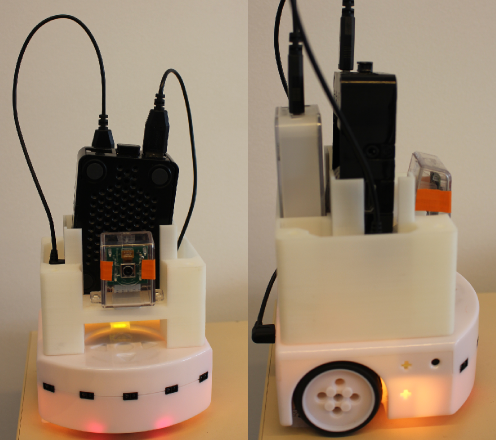
\includegraphics[scale = 0.70]{fig/Discussion/Robot.png}
	          \caption{\textbf{Physical robot for distributed robotics.}
	          Picture of a robot designed to be used for our experiments in distributed robotics. This robot is composed of a Thymio-II base which is equipped with two wheels and a collection of sensors, among which proximity sensors. A 3D-printed structure is used to support a raspberry PI, a camera module and a battery. The raspberry PI is used to have a more complex control of the Thymio.} 
	          \label{fig:thymioPicture}
	        \end{center}
	    \end{figure}

			As such one perspective could potentially be to apply or evolved solution in these real robots. This point might relate to both parts of this thesis. However, in the case of modeling the evolution of cooperation, we would not learn more by using real robots rather than simulated ones. As previously explained, this would mostly ensure that no unrealistic physical assumptions are made in our simulations. We thus believe real robots to be more of an interesting perspective in our study of automatic design in evolutionary robotics. Preliminary experiments on those robots showed that the evolved leader/follower strategy could transfer well in simple situations. Additional experiments are needed to really validate the transferability of our solutions.

\section{Concluding Remarks}

	The present work aimed at contributing to the field of evolutionary robotics in two different ways: model and design~\parencite{Trianni2014b, Doncieux2015a}. On the one hand, we modeled the evolution of mutualistic cooperation. Thanks to evolutionary robotics we could show that the proximate aspect of behaviours are critical in understanding the origin of mutually beneficial actions. On the other hand, we studied the automatic design of controllers for distributed robotics. We revealed that there are advantages in using heterogeneous teams of individuals and that it may be useful no to restort to the classical approach of evolving clonal controllers. In conclusion, we want to insist on the fact that research on these two aspects of evolutionary robotics has to be done separately. In it necessary to clearly state to which direction each work contribution. However, as we showed here, benefits can be extracted by taking inspiration from one side to the other. 

	% Therefore we contributed to the open question of genetic team compositions in evolutionary robotics. In conclusion we believe that evolutionary robotics can indeed seriously contribute in one or the other way and that there is potential for scientific research in either direction.

	% Thus we hopped to convince readers that there is an interest in using evolutionary robotics as a modeling framework in evolutionary biology and that a wide range of other phenomena could be adressed this way
